\lab{Algorithms}{Interior Point I}{Interior Point I}
\objective{Learn About Interior Point Methods for Linear Programming}

\section*{Interior Point Methods: Overview}
Although the Simplex algorithm was long the only practically competitive method for linear programming, the past 30 years have seen the discovery and widespread adoption of a new family of algorithms that rival and in some cases outperform the Simplex algorithm, collectively called Interior Point methods. One of the major shortcomings of the Simplex algorithm is that the number of steps required to solve the problem can grow exponentially in the size of the linear system. Thus, for certain large linear programs, the Simplex algorithm is simply not viable. In practice, however, such pathological examples are rarely encountered. Interior Point methods offer and alternative approach and guarantee much better theoretical convergence properties.

Recall that a linear program is a constrained optimization problem with a linear objective function and linear constraints.
The linear constraints define a set of allowable points called the \emph{feasible region}, the boundary of which forms a geometric
object known as a \emph{polytope}. The theory of convex optimization ensures that the optimal point for the objective function
can be found among the vertices of the feasible polytope. The Simplex Method tests a sequence of such vertices until it finds
the optimal point. Provided the linear program is neither unbounded nor infeasible, the algorithm is certain to produce the correct
answer after a finite number of steps, but it does not guarantee an efficient path along the polytope toward the minimizer. Interior point methods do away with the feasible polytope and instead generate a sequence of points that cut through the interior (or
exterior) of the feasible region and converge iteratively to the optimal point. Although it is computationally more expensive to
compute such interior points, each step results in significant progress toward the minimizer. See Figure \ref{fig:intPath} for
a visualization of an Interior Point method. In general, the Simplex Method requires many more, albeit less expensive, computations.

\begin{figure}
\centering
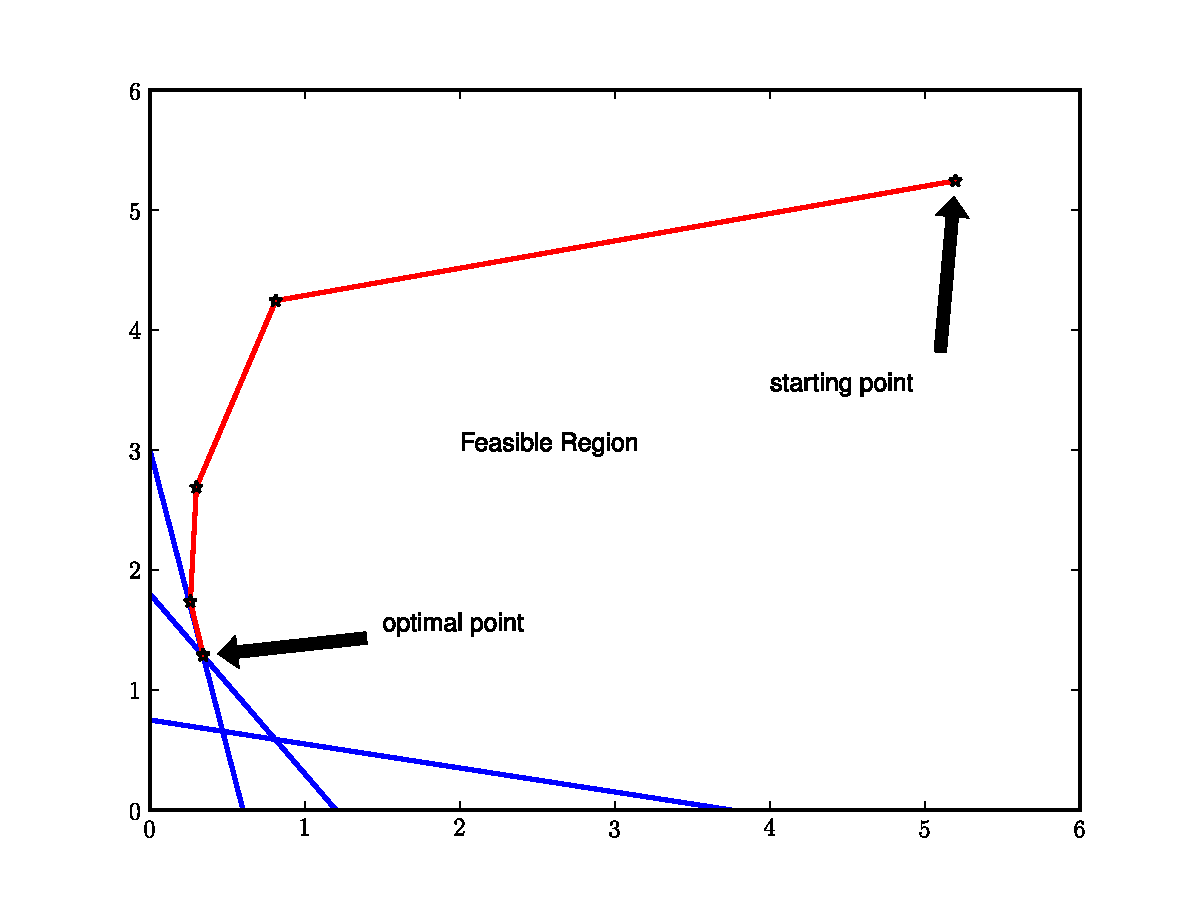
\includegraphics[width=\textwidth]{interiorPath.pdf}
\caption{A path traced by an Interior Point algorithm.}
\label{fig:intPath}
\end{figure}

\section*{Primal-Dual Interior Point Methods}
Some of the most popular and successful types of Interior Point methods nowadays are known as Primal-Dual Interior Point methods. To
describe this approach, let us consider the following linear program:
\begin{align*}
\text{minimize }\qquad &c^Tx\\
\text{subject to }\qquad &Ax = b\\
&x \geq 0.
\end{align*}
Here, $x, c \in \mathbb{R}^n$, $b \in \mathbb{R}^m$, and $A$ is an $m \times n$ matrix with full row rank. By $x \geq 0$, we
simply mean that each coordinate of $x$ is nonnegative. Note that this formulation is quite general, as any linear program can be
posed in this manner, after appropriate transformations. This is the primal problem, and its dual takes the form
\begin{align*}
\text{maximize } &b^T\lambda\\
\text{subject to } &A^T\lambda + s = c\\
&s \geq 0,
\end{align*}
where $\lambda \in \mathbb{R}^m$ and $s \in \mathbb{R}^n$. The theory of convex optimization gives us necessary and sufficient
conditions for the solutions to the primal and dual problems via the Karush-Kuhn-Tucker conditions, which in this case take the form
\begin{align*}
A^T\lambda + s &= c\\
Ax &= b\\
x_is_i &= 0, \,\,\, i = 1,2,\ldots,n\\
x, s &\geq 0.
\end{align*}
A Primal-Dual Interior Point method is a line search method that starts with an initial guess $(x_0, \lambda_0, s_0)$
and produces a sequence of points that converge to $(x^*, \lambda^*, s^*)$, the solution to the KKT equations and hence
the solution to the original linear program.

\subsection*{Search Direction and Step Length}
We now describe how to select the search direction and step length at each iteration of the algorithm. Because this is
a constrained problem, matters are more complicated than is usual in unconstrained line search methods.

The top three lines of the KKT conditions can be rewritten as one large almost-linear homogeneous system of equations.
In the spirit of
Newton's Method, we can form a linear approximation of this system centered around our current point $(x, \lambda, s)$, and
calculate the direction $(\triangle x, \triangle \lambda, \triangle s)$ in which to step in order to set the linear approximation
equal to 0. This equates to solving the linear system
\begin{equation}
\begin{bmatrix}
0 & A^T & I\\
A & 0 & 0\\
S & 0 & X
\end{bmatrix}
\begin{bmatrix}
\triangle x\\
\triangle \lambda\\
\triangle s
\end{bmatrix}
=
\begin{bmatrix}
-r_c\\
-r_b\\
-XSe
\end{bmatrix},
\label{eq:affine}
\end{equation}
where $r_b = Ax - b,$ $r_c = A^T\lambda + s - c$, $I$ is an appropriately-sized identity matrix, $X = \text{diag}(x_1,\ldots,x_n),$
$S = \text{diag}(s_1,\ldots,s_n)$, and $e = (1,1,\ldots,1)^T$.
This Newton direction is too greedy, however, and even small steps in this direction may cause us to violate the nonnegativity
condition (the last line of the KKT conditions). We need to find a new search direction.

Choosing an appropriate search direction is a tricky task, and various approaches exist. We will follow a popular strategy
known as the \emph{Predictor-Corrector Algorithm}. The idea is to actually calculate two directions. We first calculate
the standard Newton direction described above; that is, we obtain the solution to Equation \ref{eq:affine}. This is known as
the \emph{predictor step}, since it gives us a direction in which the objective does indeed decrease, hence predicting our
final search direction. Denote the solution to this system by $(\triangle x^a, \triangle \lambda^a, \triangle s^a)$.
As discussed, however, we must deviate from this direction somewhat, and so we additionally solve the
following linear system of equations:
\begin{equation}
\begin{bmatrix}
0 & A^T & I\\
A & 0 & 0\\
S & 0 & X
\end{bmatrix}
\begin{bmatrix}
\triangle x\\
\triangle \lambda\\
\triangle s
\end{bmatrix}
=
\begin{bmatrix}
-r_c\\
-r_b\\
-XSe - \triangle X^a\triangle S^ae + \sigma \mu e
\end{bmatrix}.
\label{eq:centering}
\end{equation}
The solution to this system, which we denote by $(\triangle x, \triangle \lambda, \triangle s)$, is our final search direction.
Note that $\triangle X^a = \text{diag}(\triangle x_1^a,\ldots,\triangle x_n^a)$, $\triangle S^a = \text{diag}(\triangle s_1^a,\ldots,\triangle s_n^a)$. Further, define $\mu := x^Ts/n$. The formula for $\sigma$ is somewhat more complicated, and
is based on a heuristic approach. Make the following calculations:
\begin{align*}
\alpha_a^p &:= \min\left(1, \displaystyle\min_{i : \triangle x_i^a < 0}-\frac{x_i}{\triangle x_i^a}\right)\\
\alpha_a^d &:= \min\left(1, \displaystyle\min_{i : \triangle s_i^a < 0}-\frac{s_i}{\triangle s_i^a}\right).
\end{align*}
Next, define
$$
\mu_a := \frac{1}{n}(x+\alpha_a^p\triangle x^a)^T(s+\alpha_a^d\triangle s^a).
$$
Finally, calculate $\sigma$ by the formula
$$
\sigma = \left(\frac{\mu_a}{\mu}\right)^3.
$$

Now that we have our search direction, it remains to choose our step length. We wish to step nearly as far as possible without
violating the nonnegativity condition, thus remaining in the interior of the feasible region. First, make the following
calculations:
\begin{align*}
\beta^p &:= \displaystyle\min_{i : \triangle x_i < 0}-\frac{x_i}{\triangle x_i}\\
\beta^d &:= \displaystyle\min_{i : \triangle s_i < 0}-\frac{s_i}{\triangle s_i}.
\end{align*}
Next, calculate
\begin{align*}
\alpha^p &:= \min(1, 0.95\beta^p)\\
\alpha^d &:= \min(1, 0.95\beta^d).
\end{align*}
These are our step lengths. That is, our next point $(x', \lambda', s')$ is given by
\begin{align*}
x' &= x + \alpha^p\triangle x\\
(\lambda', s') &= (\lambda, s) + \alpha^d(\triangle \lambda, \triangle s).
\end{align*}
We summarize the entire procedure in Algorithm \ref{alg:predcorr}.
\begin{algorithm}
\begin{algorithmic}[1]
\Procedure{Predictor-Corrector Algorithm}{}
    \State \textrm{Choose initial point } $(x_0, \lambda_0, s_0)$.
    \For{$k = 0, 1, 2, \ldots$}
        \State \textrm{Solve for } $(\triangle x^a, \triangle \lambda^a, \triangle s^a)$.
        \State \textrm{Calculate } $\alpha_a^p, \alpha_a^d, \mu_a$, \textrm{and} $\sigma$.
        \State \textrm{Solve for } $(\triangle x, \triangle \lambda, \triangle s)$.
        \State \textrm{Calculate the step lengths } $\alpha^p, \alpha^d$.
        \State $x_{k+1} = x_k + \alpha^p\triangle x$,\\
        $\qquad\quad(\lambda_{k+1}, s_{k+1}) = (\lambda_k, s_k) + \alpha^d(\triangle \lambda, \triangle s)$.
    \EndFor
\EndProcedure
\end{algorithmic}
\caption{Predictor-Corrector Algorithm}
\label{alg:predcorr}
\end{algorithm}

A few notes on the implementation of this algorithm are in order. 
In each iteration, by far the most expensive operations are solving Equations \ref{eq:affine} and 
\ref{eq:centering}. Fortunately, the only difference between the two equations is the right-hand side.
Thus, we can avoid repetitious calculation by first factorizing the block matrix
\[
\begin{bmatrix}
0 & A^T & I\\
A & 0 & 0\\
S & 0 & X
\end{bmatrix}
\]
once at the beginning of the iteration, and then using the factorization twice to solve both equations.
For convenience, consider using the functions \li{lu_factor} and \li{lu_solve} in the \li{scipy.linalg}
module. It is possible to speed up these calculations further, but for simplicity we won't pursue the issue
farther.

Next, the value of $\mu$ (defined above) gives a measure of how close our current point is to the minimizer.
The closer $\mu$ is to 0, the closer we are to the optimal point. Thus, by printing the value of $\mu$ at
each iteration, you can track how your algorithm is progressing and detect when you have converged.

Another potentially tricky calculation that comes up in each iteration has the following form:
\[
\min\left(1, \displaystyle\min_{i : u_i < 0}-\frac{v_i}{u_i}\right),
\]
where $\mathbf{u} = (u_1, \ldots, u_n)^T$ and $\mathbf{v} = (v_1, \ldots, v_n)^T$ are vectors.
This can be done in a vectorized fashion in Python as follows (assuming that the arrays \li{u} and \li{v}
have already been initialized):
\begin{lstlisting}
>>> mask = u < 0
>>> if np.any(mask):
>>>     myMin = min(1, (-v/u)[mask].min())
>>> else:
>>>     myMin = 1
\end{lstlisting}
We need the if-statement to deal with the case where no entry of $u$ is negative.

Finally, the choice of initial point $(x_0, \lambda_0, s_0)$ is an important, nontrivial one. 
A naively or randomly chosen initial point may cause the algorithm to fail to converge.
We provide code to calculate an appropriate initial point. You should include a call to this function in your algorithm to obtain the initial point.

\begin{lstlisting}
def startingPoint(A, b, c):
    """
    Calculate an initial guess to the solution of the
    linear program min c^T x, Ax = b, x>=0.
    Inputs:
        A -- array of shape (m,n) with linearly independent rows
        b -- array of length m
        c -- array of length n
    Returns:
        x -- array of length n
        lam -- array of length m
        s -- array of length n
    Ref: Nocedal and Wright, p. 410
    """
    # first calculate x, lam, s of minimal norm satisfying the primal and dual constraints
    B = la.inv(A.dot(A.T))
    x = A.T.dot(B.dot(b))
    lam = B.dot(A.dot(c))
    s = c - A.T.dot(lam)

    # perturb x and s so they are nonnegative
    dx = max((-3./2)*x.min(), 0)
    ds = max((-3./2)*s.min(), 0)
    x += dx*np.ones(x.shape)
    s += ds*np.ones(s.shape)

    # perturb x and s so they are not too close to zero, not too dissimilar
    dx = .5*(x*s).sum()/s.sum()
    ds = .5*(x*s).sum()/x.sum()
    x += dx*np.ones(x.shape)
    s += ds*np.ones(s.shape)

    return x, lam, s
\end{lstlisting}

\begin{problem}
Write a function \li{interiorPoint} that implements the interior point method described above.
The function should accept $A$, $b$, and $c$ as parameters, along with keyword arguments
\li{niter} that gives the number of iterations to perform, and \li{verbose} that indicates
whether to print out the value of the objective function and $\mu$ at each iteration.
The function should return the optimal point $x$ along with the value of the objective function at this
point.
\end{problem}
\section*{Least Absolute Deviations}
We now return to the familiar problem of fitting a line (or hyperplane) to a set of data. We have previously approached this
problem by minimizing the sum of the squares of the errors between the data points and the line, an approach known as \emph{least
squares}. The least squares solution can be obtained analytically when fitting a linear function, or through a number of optimization
methods (such as Conjugate Gradient) when fitting a nonlinear function.

The method of least absolute deviations also seeks to find a best fit line to a set of data, but the error between the data and
the line is measured differently. In particular, suppose we have a set of data points $(y_1, \mathbf{x}_1), (y_2, \mathbf{x}_2), \ldots,
(y_m, \mathbf{x}_m)$, where $y_i \in \mathbb{R}$, $\mathbf{x}_i \in \mathbb{R}^n$ for $i = 1, 2, \ldots, m$. Here, the $\mathbf{x}_i$ vectors
are the explanatory variables and the $y_i$ values are the response variables, and we assume the following linear model:
\[
y_i = \beta^T\mathbf{x}_i + b, \qquad i = 1, 2, \ldots, m,
\]
where $\beta\in\mathbb{R}^n$ and $b \in \mathbb{R}$. The error between the data and the proposed linear model is given by
\[
\sum_{i=1}^n |\beta^T\mathbf{x}_i + b - y_i|,
\]
and we seek to choose the parameters $\beta, b$ so as to minimize this error.

Before we explore how to solve this problem, a discussion of the differences between least absolute deviations and least squares is in order.
The most prominent difference between these two approaches is how they respond to outliers in the data. Least absolute deviations is
robust in the presence of outliers, meaning that one (or a few) errant data points won't severely affect the fitted line. Indeed, in most cases,
the best fit line is guaranteed to pass through at least two of the data points.
This is a desirable property when the outliers may be ignored (perhaps because they are due to measurement error or corrupted data).
Least squares, on the other hand,
is much more sensitive to outliers, and so is the better choice when outliers cannot be dismissed. See Figure \ref{fig:leastAbsDev}.

\begin{figure}
\centering
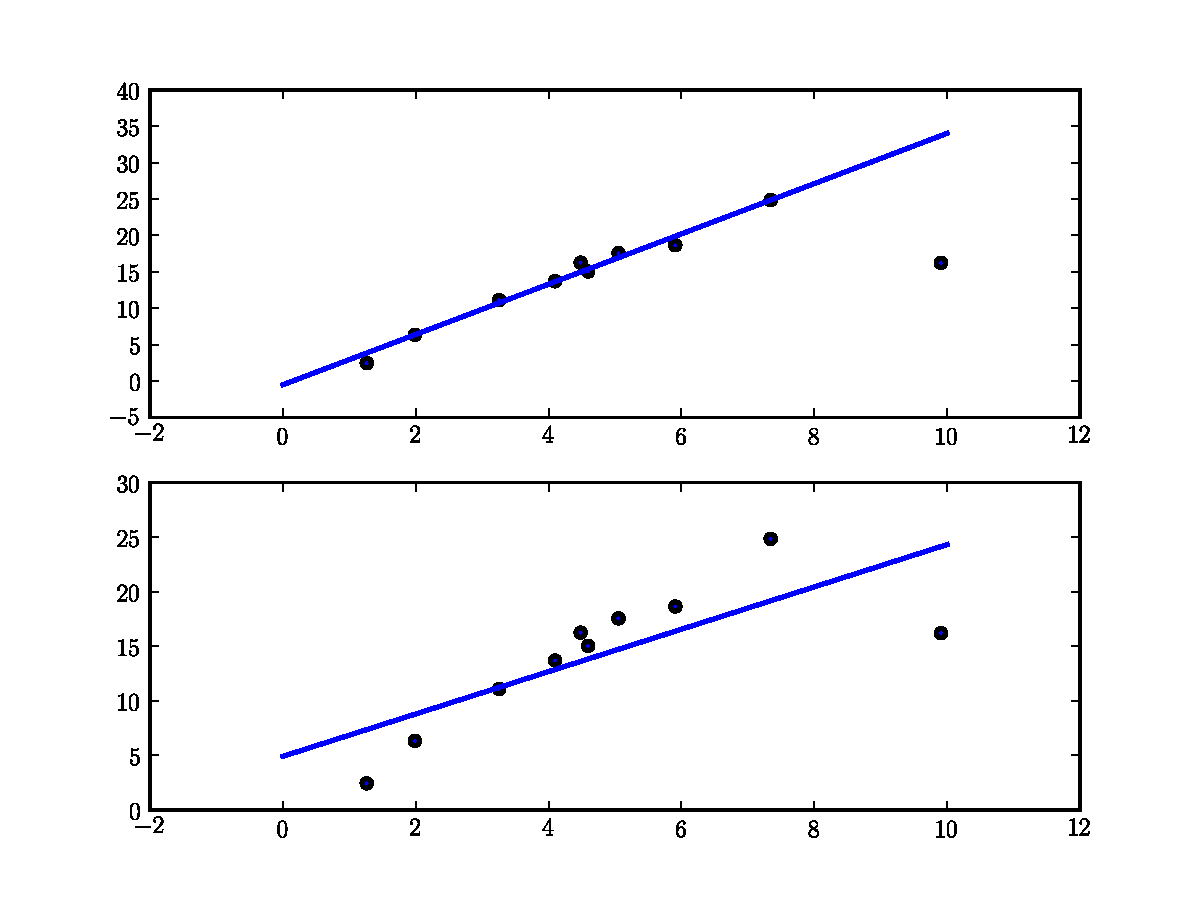
\includegraphics[width=\textwidth]{leastAbsDev.pdf}
\caption{Fitted lines produced by least absolute deviations (top) and least squares (bottom). The presence of an outlier accounts for the
stark difference between the two lines.}
\label{fig:leastAbsDev}
\end{figure}

While least absolute deviations is robust with respect to outliers, small horizontal perturbations of the data points can lead to very different
fitted lines. Hence, the least absolute deviations solution is less stable than the least squares solution. In some cases there are even infinitely
many lines that minimize the least absolute deviations error term. However, one can expect a unique solution in most cases.

The least absolute deviations solution arises naturally when we assume that the residual terms $\beta^T\mathbf{x}_i + b - y_i$ have a particular
statistical distribution (the Laplace distribution). Ultimately, however, the choice between least absolute deviations and least squares depends on the
nature of the data at hand, as well as your own good judgment.

\subsection{Least Absolute Deviations as a Linear Program}
We can formulate the least absolute deviations problem as a linear program, and then solve it using our interior point method.
For $i = 1, 2, \ldots, m$ we introduce the artificial variable $u_i$ to take the place of the error term $|\beta^T\mathbf{x}_i + b - y_i|$,
and we require this variable to satisfy $u_i \geq |\beta^T\mathbf{x}_i + b - y_i|$. This constraint is not yet linear, but we can split it into
an equivalent set of two linear constraints:
\begin{align*}
u_i &\geq \beta^T\mathbf{x}_i + b - y_i,\\
u_i &\geq y_i - \beta^T\mathbf{x}_i - b.
\end{align*}
Clearly, the $u_i$ are implicitly constrained to be nonnegative.

Our linear program can now be stated as follows:
\begin{align*}
\text{minimize }\qquad &\sum_{i=1}^m u_i\\
\text{subject to }\qquad &u_i \geq \beta^T\mathbf{x}_i + b - y_i,\\
&u_i \geq y_i - \beta^T\mathbf{x}_i - b.
\end{align*}
This is not yet in the form that we need in order to use our interior point method.
For each inequality constraint, we bring all variables ($u_i, \beta, b$) to the left hand side and
introduce a nonnegative slack variable to transform the constraint into an equality:
\begin{align*}
u_i  - \beta^T\mathbf{x}_i - b - s_{2i}&= -y_i,\\
u_i +\beta^T\mathbf{x}_i + b - s_{2i+1}&= y_i,\\
s_{2i}, s_{2i+1}&\geq 0.
\end{align*}

Notice that the variables $\beta, b$ are not assumed to be nonnegative, but in our interior point method, all variables are assumed
to be nonnegative. We can fix this situation by writing these variables as the difference of nonnegative variables:
\begin{align*}
  \beta &= \beta_1 - \beta_2,\\
  b &= b_1 - b_2,\\
  &\beta_1, \beta_2, b_1, b_2 \geq 0.
\end{align*}
Substituting these values into our constraints, we have the following system of constraints:
\begin{align*}
u_i  - \beta_1^T\mathbf{x}_i + \beta_2^T\mathbf{x}_i - b_1 + b_2 - s_{2i}&= -y_i,\\
u_i + \beta_1^T\mathbf{x}_i - \beta_2^T\mathbf{x}_i + b_1 - b_2 - s_{2i+1}&= y_i,\\
u_i, \beta_1, \beta_2, b_1, b_2, s_{2i}, s_{2i+1}&\geq 0.
\end{align*}
Writing $\mathbf{y} = (-y_1, y_1, -y_2, y_2, \ldots, -y_m, y_m)^T$ and $\beta_i = (\beta_{i,1}, \ldots, \beta_{i,n})^T$ for $i = 1, 2$,
we can aggregate all of our variables into one vector as follows:
\[
\mathbf{v} = (u_1,\ldots, u_m, \beta_{1,1},\ldots, \beta_{1,n}, \beta_{2,1},\ldots, \beta_{2,n}, b_1, b_2, s_1,\ldots,s_{2m+1})^T.
\]
Defining $\mathbf{c} = (1, 1, \ldots, 1, 0, \ldots, 0)^T$ (where only the first $m$ entries are equal to 1), we can write our
objective function as
\[
\sum_{i=1}^m u_i = \mathbf{c}^T\mathbf{v}.
\]
Hence, the final form of our linear program is
\begin{align*}
  \text{minimize }\qquad &\mathbf{c}^T\mathbf{v}\\
  \text{subject to }\qquad A\mathbf{v} &= \mathbf{y},\\
  \mathbf{v} &\geq 0,
\end{align*}
where $A$ is a matrix containing the coefficients of the constraints.
Our constraints are now equalities, and the variables are all nonnegative, so we are ready to use our interior point method to obtain
the solution.

Let's work through an example. We start with an array \li{data}, each row of which consists of the values $y_i, x_{i,1},\ldots,x_{i,n}$,
where $\mathbf{x}_i = (x_{i,1}, x_{i,2}, \ldots, x_{i,n})^T$. We will have $3m + 2(n+1)$ variables in our linear program. Below, we initialize
the vectors $\mathbf{c}$ and $\mathbf{y}$.
\begin{lstlisting}
>>> m = data.shape[0]
>>> n = data.shape[1] - 1
>>> c = np.zeros(3*m + 2*(n + 1))
>>> c[:m] = 1
>>> y = np.empty(2*m)
>>> y[::2] = -data[:, 0]
>>> y[1::2] = data[:, 0]
>>> x = data[:, 1:]
\end{lstlisting}

The hardest part is initializing the constraint matrix correctly. It has $2m$ rows and $3m + 2(n+1)$ columns. Try writing out the
constraint matrix by hand for small $m, n$, and make sure you understand why the code below is correct.
\begin{lstlisting}
>>> A = np.ones((2*m, 3*m + 2*(n + 1)))
>>> A[::2, :m] = np.eye(m)
>>> A[1::2, :m] = np.eye(m)
>>> A[::2, m:m+n] = -x
>>> A[1::2, m:m+n] = x
>>> A[::2, m+n:m+2*n] = x
>>> A[1::2, m+n:m+2*n] = -x
>>> A[::2, m+2*n] = -1
>>> A[1::2, m+2*n+1] = -1
>>> A[:, m+2*n+2:] = -np.eye(2*m, 2*m)
\end{lstlisting}

Now we can calculate the solution by calling our interior point function.
\begin{lstlisting}
>>> sol = interiorPoint(c, A, y, niter=10, verbose=False)[0]
\end{lstlisting}

The variable \li{sol}, however, holds the value for the vector
\[
\mathbf{v} = (u_1,\ldots, u_m, \beta_{1,1},\ldots, \beta_{1,n}, \beta_{2,1},\ldots, \beta_{2,n}, b_1, b_2, s_1,\ldots,s_{2m+1})^T.
\]
We want the values of $\beta = \beta_1-\beta_2$ and $b = b_1 - b_2$, and we accomplish this by the
following code:
\begin{lstlisting}
>>> beta = sol[m:m+n] - sol[m+n:m+2*n]
>>> b = sol[m+2*n] - sol[m+2*n+1]
\end{lstlisting}

\begin{problem}
The file \li{simdata.txt} contains two columns of data. The first gives the values of the response
variables, and the second column gives the values of the explanatory variables. Find the least absolute
deviations line for this data set, and plot it together with the data.
\end{problem} 